\section{Deployment}\label{sec:03_depl}
% Explain section
This section explains the deployment of the application.
% Requirements
The only requirement to run this application, is to have tomcat 9 installed.

\Fig{fig:subsubsec:03_depl_process} illustrates the process of deploying the \path{ROOT.war} file using tomcat.
\begin{figure}[h]
\centering
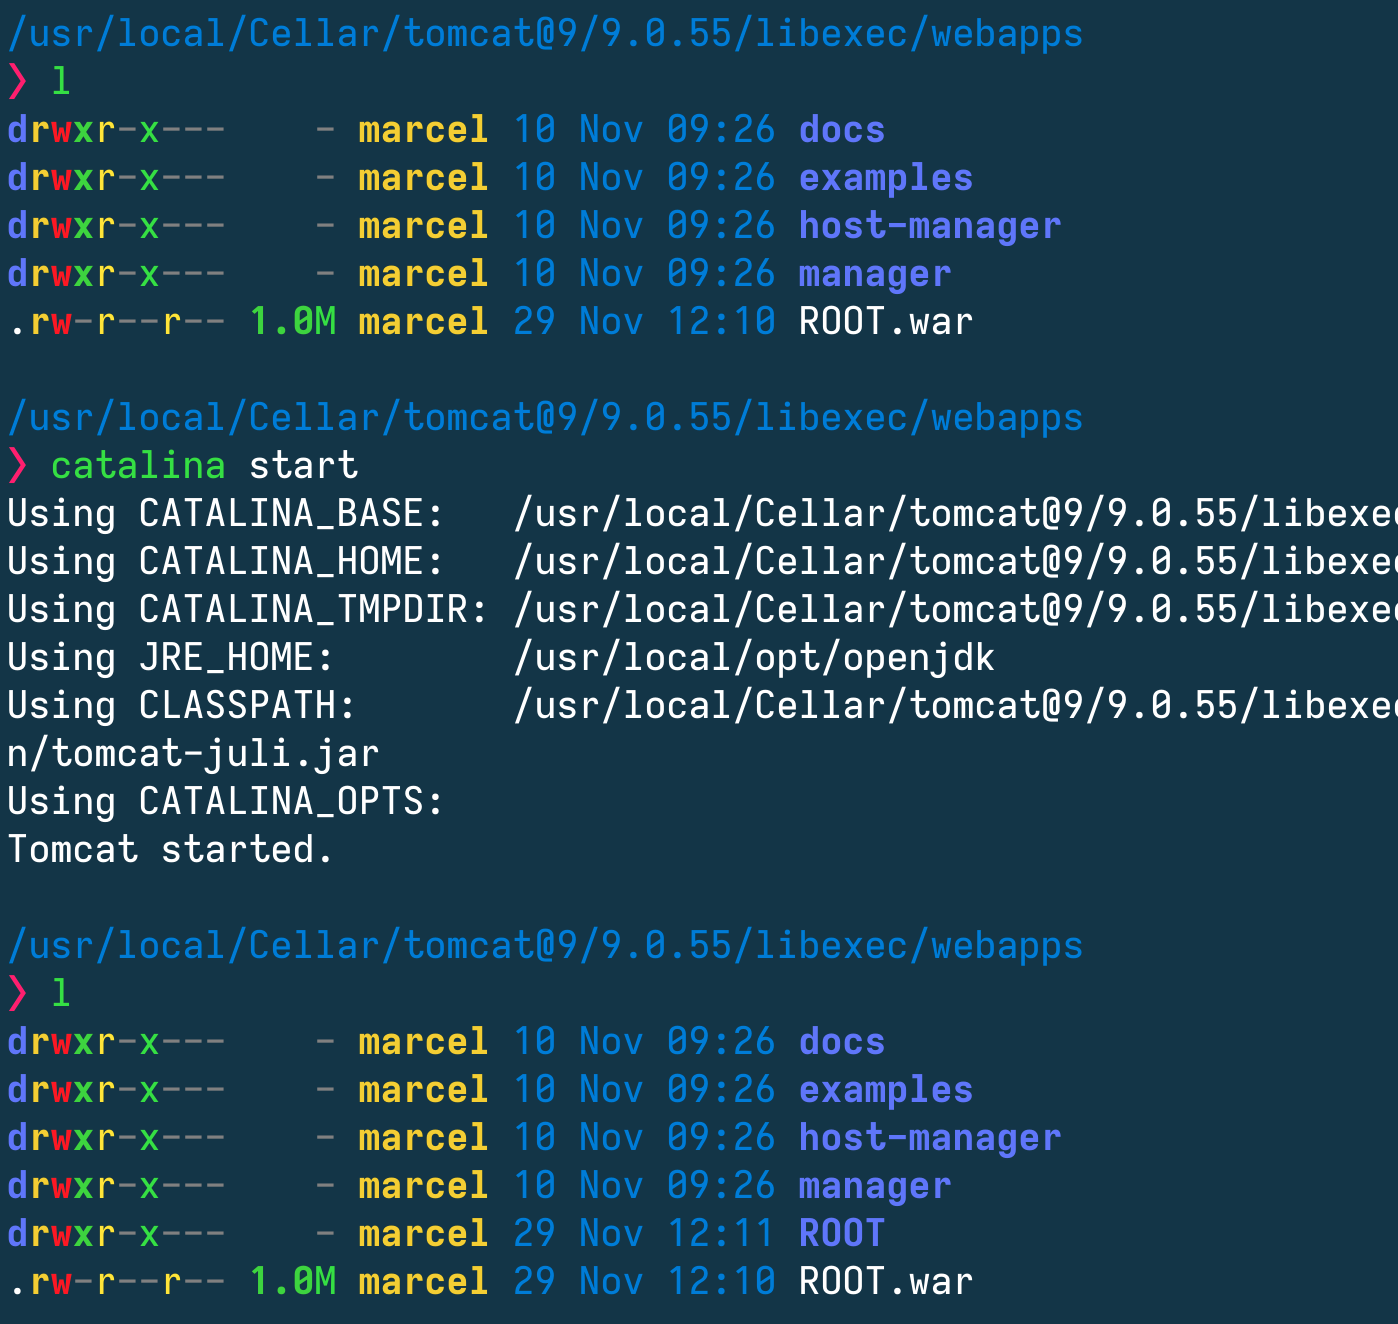
\includegraphics[scale=0.5]{images/03_depl/process}
\caption{Deployment process using \texttt{ROOT.war}}
\label{fig:subsubsec:03_depl_process}
\end{figure}

\paragraph{1.}
The first step, is to copy the \path{ROOT.war} file to the \path{webapps/} folder of the tomcat installation.
This can be done using \texttt{\$ cp ROOT.war TOMCAT\_DIRECTORY/webapps}.

\paragraph{2.}
Next, the remaining step is to start the tomcat server using \texttt{catalina start}. Tomcat will automatically extract the \path{ROOT.war} to a directory called \path{ROOT/}.

\paragraph{3.}
After that, the application is available via \url{http://localhost:8080/}.
